\documentclass[10pt,landscape]{cheatsheet}

\usepackage{lipsum}
\usepackage[labelfont=bf]{caption}
\usepackage{fontspec}

\setmainfont{Latin Modern Roman}

\begin{document}
\footnotesize
\begin{multicols}{3}

\begin{center}
     \Large{\textbf{Rubik's Cheatsheet}} \\
     Luke Hsiao
\end{center}

\section{Notation}
\begin{Figure}
    \centering
    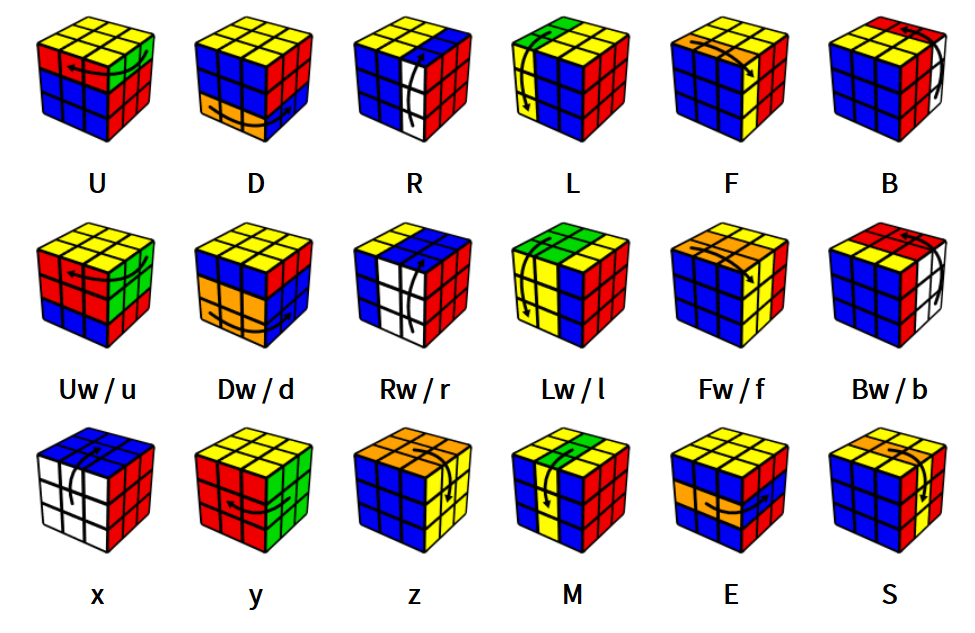
\includegraphics[width=\linewidth]{img/notation.png}
    \captionof{figure}{%
        Each notation corresponds to a clockwise turn if you were looking at the face.
        M, E, and S follow the face that they are closest alphabetically to.
    }\label{fig:notation}
\end{Figure}

\lipsum[1]

\newcommand{\mitem}[2]{#1 & #2 \\}
\begin{tabular}{@{}ll@{}}
    \mitem{Pellentesque}{Eget nisl ut lorem fringilla elementum.}
    \mitem{Curabitur}{Consequat nisi at ligula hendrerit condimentum.}
    \hline
    \mitem{Pellentesque}{Eget nisl ut lorem fringilla elementum.}
    \mitem{Curabitur}{Consequat nisi at ligula hendrerit condimentum.}
\end{tabular}

\end{multicols}
\end{document}
